% main_v2.tex -- camera-ready source. Every number traces to a committed artifact (REPRODUCE.md).
% Load the NeurIPS style before hyperref. No option = anonymous review mode; switch to [final]
% (plus authors and the workshop footer) only for the de-anonymised camera-ready upload.
\documentclass{article}

\IfFileExists{neurips_2026.sty}{%
  \usepackage[final]{neurips_2026}%
}{%
  \usepackage[margin=1in]{geometry}%
  \PackageWarningNoLine{main}{neurips_2026.sty not found - using fallback geometry. Page count will NOT match the official template.}%
}

\makeatletter
\renewcommand{\@noticestring}{NewInML Workshop at the 40th Conference on Neural Information Processing Systems (NeurIPS 2026), Paris, France, 2026.}
\makeatother

\usepackage[utf8]{inputenc}
\usepackage[T1]{fontenc}
\usepackage{hyperref}
\usepackage{url}
\usepackage{booktabs}
\usepackage{amsfonts}
\usepackage{nicefrac}
\usepackage{microtype}
\usepackage{xcolor}
\usepackage{graphicx}
\usepackage{amsmath}

\newcommand{\justification}[1]{#1}
\graphicspath{{../results/figures/}{figures/}}

\title{Metric-as-Feature Leakage: A Feature-Side\\
       Failure Mode in Retriever Routing}

\author{
  Soumy Sawant\\
  Manipal University Jaipur\\
  Jaipur, India\\
  \texttt{soumy.250205119@muj.manipal.edu}
  \And
  Chirag Joshi\\
  Manipal University Jaipur\\
  Jaipur, India\\
  \texttt{joshi.chirag@jaipur.manipal.edu}
}

\begin{document}
\maketitle

\begin{abstract}
Retriever routing chooses a retrieval strategy per query in retrieval-augmented generation. On
NQ, TriviaQA and HotpotQA, an oracle choosing among three retrievers per query beats the best
fixed one by 21--46\% relative. A router we built appeared to capture much of this gap until we
found that four of its features had been read from the evaluation metric, MRR@20, which equals
the reward for two retrievers whenever the answer ranks in the top 20. The correct, label-free
features scored \emph{below} a constant baseline, so every usual signal pointed toward the leak.
We use this accidental bug as a controlled case of target leakage. With the reward table fixed
and only the leaked features varied, accuracy at predicting the best retriever rises from 59.9\%
(label-free; majority 60.9\%) to 73.1\%, and a tuned router's apparent capture of the oracle gap
rises from about zero to about 70\%. The leak need not be exact: a hit-or-miss version still buys
8 points over the majority baseline, and for a gradient-boosted router, noisy versions that match
no reward value keep about half the gain under additive noise of $\pm$0.15 and essentially all of
it under multiplicative noise of $\pm$15\%, so an equality check misses them. Without the leak, no
selection method we tested beats the best fixed retriever, though our test splits can only detect
methods capturing roughly 43--72\% of the gap or more. We release \texttt{leakcheck}, an audit of
a feature matrix against a per-arm reward table, report where it fails, run it on a third party's
released router features (QueryRoute; clean), and propose a feature-provenance checklist: a
routing result should ship with the feature matrix behind it.
\end{abstract}

% =====================================================================================
\section{Introduction}
\label{sec:intro}

\emph{A routing result is only as trustworthy as the feature matrix behind it.} This paper
measures how far that can go wrong, using a mistake we made ourselves.

Retrieval-augmented generation grounds a language model in retrieved
passages~\cite{lewis2020rag}. Many pipelines use one retrieval strategy (sparse~\cite{robertson2009bm25},
dense~\cite{karpukhin2020dpr} or a fusion) for every query~\cite{stouras2026portfolios}, yet on our
benchmarks an oracle that picks the best of three retrievers per query beats the best fixed one
by 21--46\% relative. That gap motivates per-query retriever
selection~\cite{arabzadeh2021bertselect,balasubramanian2010rankers}, a case of per-instance
algorithm selection~\cite{rice1976algorithm,kerschke2019automated}.

We built a learned router for this gap, and it beat every fixed retriever. It did so because our
feature extractor read each retriever's per-query record, which holds raw label-free scores next
to evaluation metrics computed \emph{from the gold answer}, and it read the metrics. In the
reconstruction we study, the leaked value is MRR@20, which equals the reward for BM25 or Dense
whenever the answer ranks in the top 20. This is target leakage in the classical
sense~\cite{kaufman2012leakage,kapoor2023leakage}; we do not claim the category is new. Two facts
make it worth measuring rather than only fixing. The correct, label-free features score
\emph{below} a constant baseline, so the honest router looks useless while the leaked one looks
good. And the obvious audit, checking that no feature equals a reward, catches an exact copy but
not a perturbed one.

\begin{figure}[t]
\centering
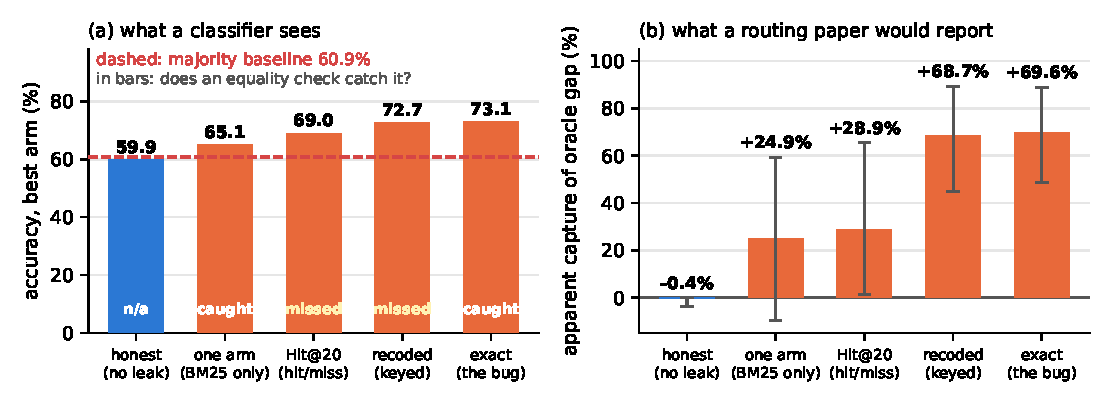
\includegraphics[width=\textwidth]{fig12_leak_ladder.pdf}
\caption{\textbf{What the leak buys.} Five feature sets that differ only in features 22--25 and
share one reward table: \emph{honest} (label-free score statistics), \emph{one arm} (BM25's
MRR@20 copied), \emph{Hit@20} (a hit-or-miss indicator instead), \emph{recoded} (MRR@20 with a
value-keyed offset of up to $\pm$0.15) and \emph{exact} (both arms' MRR@20, the original bug).
(a) Accuracy at predicting the best retriever (default gradient boosting, pooled, 3{,}175
queries); the label inside each bar says whether an equality check (a \texttt{leakcheck}
verdict) catches that leak. (b) The same leaks in the units a routing paper reports: capture of the oracle gap
by a tuned router on held-out test queries, mean over three datasets and five data splits;
whiskers show the range.}
\label{fig:ladder}
\end{figure}

We ask three questions. \textbf{RQ1} (\S\ref{sec:doseresponse}): how much outcome information
manufactures apparent routing gains, and must it be exact? \textbf{RQ2} (\S\ref{sec:results}):
what routing signal remains once it is removed? \textbf{RQ3} (\S\ref{sec:tool}): can the failure be
found by auditing the feature matrix? Our answers form the paper's three contributions:
\begin{enumerate}\setlength{\itemsep}{0pt}
  \item \textbf{A graded measurement of the leak} (Figure~\ref{fig:ladder}): from $+4.2$ to $+12.2$
    accuracy points over the majority baseline, or about 25\% to 70\% apparent capture, depending
    on how much leaks; for gradient boosting, a perturbed leak keeps from about half to all of its
    advantage.
  \item \textbf{A bounded negative result}: without the leak, nothing beats the best fixed
    retriever (best capture $+0.4\%$, 95\% interval 0.0--1.5\%), and we state what the test splits
    could have detected.
  \item \textbf{An audit tool tested against its own failure}: \texttt{leakcheck} raises suspicion
    from correlation but issues a verdict only on exact agreement, after real data falsified its
    first design; a feature-provenance checklist; and an audit of a third party's released router
    features (QueryRoute), which comes back clean.
\end{enumerate}
We show that leakage is \emph{sufficient} to manufacture routing gains, not that it is necessary:
genuine gains are reported for diverse retriever
pools~\cite{kuru2026retrievalrouter,stouras2026portfolios,six2026ragcompass}, and a synthetic
positive control shows a genuine gain next to a leaked one (\S\ref{sec:doseresponse}).

% =====================================================================================
\section{Related work}
\label{sec:related}

\paragraph{Retriever routing.} Selecting a ranker per query is long studied in
IR~\cite{balasubramanian2010rankers}. Arabzadeh et al.~\cite{arabzadeh2021bertselect} pick sparse or dense
from the query and sparse or hybrid after a sparse pass, trading recall against cost. Adaptive-RAG~\cite{jeong2024adaptiverag}
and MBA-RAG~\cite{tang2025mbarag} route between retrieval \emph{strategies} (none, single- or
multi-step) by query complexity, MBA-RAG as a bandit; RouterRetriever~\cite{campos2024routerretriever}
routes over expert embedders. LTRR~\cite{qin2024ltrr} and \mbox{R\textsuperscript{3}AG}~\cite{zhao2026r3ag}
report routing beating the best single retriever (by 1.75 EM on our three datasets for R$^3$AG),
as do RetrievalRouter~\cite{kuru2026retrievalrouter} and retriever
portfolios~\cite{stouras2026portfolios}, over deliberately diverse pools. Concurrent work that
reads the retrieved passages gains 28\% relative answer F1, while ``none of the tested query-only
routers exceeds the best fixed retriever under either shift''~\cite{six2026ragcompass}.

\paragraph{Why routers fail.} Routers ``collapse to majority-class prediction'' with headroom
``substantially inflated''~\cite{garg2026unsolvability}, converge far below the
oracle~\cite{lu2026routingplateau}, face a 94.9\% tie rate on RouterBench~\cite{lai2026routing},
and may need evidence that ``is only revealed after searching the index''~\cite{hussain2026coverage};
a commit-before-response policy and a hindsight oracle are different decision
classes~\cite{chen2026routinggap}. These explain why a router fails. We study why one can
\emph{appear} to succeed.

\paragraph{Leakage.} Kaufman et al.~\cite{kaufman2012leakage} define leakage as target information
in inputs that would not legitimately be available at prediction time; our decision-time boundary
(\S\ref{sec:setup}) is their ``learn--predict separation'' applied to a per-arm reward table
(finance calls it look-ahead bias). Kapoor and Narayanan~\cite{kapoor2023leakage} leave their
category [L2], ``model uses features that are not legitimate'', undivided, and
Roth~\cite{roth2026leakagetypes} measures only procedural classes. Perturbed leaks are known to
matter: noise-added leaks are detected in forecasting~\cite{talagala2024tsdataleaks}, ``noisy proxies
of the target can cause substantial inflation'' at one noise level~\cite{bioleak2026}, and graded
target-derived columns degrade in-context learning~\cite{upendra2026supportset}. Detectors read
pipeline code~\cite{leakagedetector2025} or a single target~\cite{bioleak2026}. We know of no graded
measurement of what a leaking feature is worth under which perturbation for a per-arm reward
table, and no detector that takes such a table.

% =====================================================================================
\section{Setup}
\label{sec:setup}

\paragraph{The decision-time boundary.} A router commits before it sees the outcome, so its
features may use only the query and statistics of retriever outputs computed without the gold
answer. Both kinds of number sit in the same per-query record, and nothing marks the boundary
between them (Table~\ref{tab:record}). Crossing it is target leakage, with a table of per-arm
rewards in place of a single label. In our pipeline the crossing was one dictionary key.

\begin{table}[t]
\centering
\small
\caption{\textbf{Anatomy of the bug.} Top: the fields of one retriever's per-query record, as our
retrieval stage wrote them. Bottom: the line that built feature 22 before and after the fix
(feature 23 is the same line for Dense). Both versions run without error and produce a plausible
number; only one is available when the router decides.}
\label{tab:record}
\begin{tabular}{p{0.44\textwidth}p{0.48\textwidth}}
\toprule
\textbf{Label-free: usable at decision time} & \textbf{Computed from the gold answer: evaluation only} \\
\midrule
\texttt{top1\_score}, \texttt{mean\_score\_top5}, \texttt{std\_score\_top5}, \texttt{scores\_top10},
\texttt{retrieved\_ids\_top10}, \texttt{latency\_ms}
& \texttt{gold\_rank}; \texttt{metrics\_at\_k}: hit, MRR, recall, F1 and EM at $k\in\{1,3,5,10,20\}$ \\
\midrule
\multicolumn{2}{l}{\footnotesize Leaked:\; \texttt{avg\_bm25 = float(bm25\_k\_metrics.get("mrr", 0.0))}} \\
\multicolumn{2}{l}{\footnotesize Fixed:\;\;\, \texttt{f22 = float(bm25\_m.get("mean\_score\_top5", bm25\_m.get("top1\_score", 0.0)))}} \\
\bottomrule
\end{tabular}
\end{table}

\paragraph{Data, arms and reward.} NQ, TriviaQA and HotpotQA (1{,}157 / 1{,}539 / 916 queries with
a real Wikipedia gold passage). Each query is scored against 500 passages from a shared pool of
100{,}000: one gold passage (containing the answer string) and 499 distractors, about half mined
for query-term overlap and half random. The arms are BM25 ($k_1{=}1.5$, $b{=}0.75$), Dense
(\texttt{all-MiniLM-L6-v2}~\cite{reimers2019sentence}, whose fine-tuning data include NQ and
TriviaQA questions) and Hybrid (reciprocal rank fusion~\cite{cormack2009rrf}, $k{=}60$). An
arm's reward is the reciprocal rank of the first answer-bearing passage. Table~\ref{tab:arms}
shows that Dense wins on average everywhere: Hybrid trails it by 5--24\%, RRF being sensitive to
unequal inputs~\cite{bruch2023fusion,benham2017riskreward}, and BM25 is handicapped by the
overlap-mined distractors, which also deflate the query terms' IDF because it is computed per
candidate set. With a full collection, hybrid beats dense~\cite{ma2021replication}; on our shared
100K-passage index (\S\ref{sec:doseresponse}) Hybrid is the best fixed arm on TriviaQA and
HotpotQA, where BM25 also beats Dense. Our conclusions are about routing over \emph{these} arms.

\paragraph{Features and protocol.} 61 features: 29 handcrafted (lexical, entity, structural, and
seven label-free retrieval statistics, of which indices 22--25 are score features) and 32
principal components of the query embedding, fit on the training split; the same components
enter every feature set we compare, so they cancel in every premium. One fixed 70/15/15 split
serves every method. Every
arm's reward is observed on every training query, so training is offline cost-sensitive
learning, not bandit feedback.

\paragraph{Terms.} \emph{Headroom} is the oracle's mean reward minus the best fixed arm's;
\emph{capture} is the share of it a method recovers, from 0\% (best fixed) to 100\% (oracle), the
closed-gap measure of algorithm selection~\cite{lindauer2019ascompetitions}. Accuracy differences
are percentage \emph{points}: \emph{lift} is over the majority baseline, \emph{premium} over the
label-free (honest) features, and \emph{retention} is a perturbed leak's premium as a share of the
exact leak's.

\begin{table}[t]
\centering
\small
\caption{The arms and the per-query oracle on the test split (reciprocal rank of the first
answer-bearing passage). Bold: best fixed arm. Headroom is 21\%, 35\% and 46\% relative.}
\label{tab:arms}
\begin{tabular}{lrrrr}
\toprule
& BM25 & Dense & Hybrid & Oracle \\
\midrule
NQ       & 0.103 & \textbf{0.166} & 0.146 & 0.200 \\
TriviaQA & 0.150 & \textbf{0.200} & 0.191 & 0.269 \\
HotpotQA & 0.047 & \textbf{0.075} & 0.057 & 0.110 \\
\bottomrule
\end{tabular}
\end{table}

% =====================================================================================
\section{RQ1: How much does the leak buy?}
\label{sec:doseresponse}

\textbf{Takeaway: a leaked metric manufactures most of an oracle gap, and it does not have to be
exact.}

\paragraph{The leak ladder.} We build five feature sets that differ \emph{only} in features
22--25 and verify that the reward table is byte-identical across them. \emph{Honest} uses raw
top-5 score statistics. \emph{One arm} leaks BM25's MRR@20 only. \emph{Hit@20} leaks a hit-or-miss
indicator instead of the value. \emph{Recoded} adds an offset of up to $\pm$0.15 keyed on the
value, so equal values stay equal. \emph{Exact} copies both arms' MRR@20, the original bug; it equals the reward on
26--45\% of rows and is 0 otherwise. The rungs vary how many arms leak and how faithfully, so they
form an ordered ladder rather than a scalar dose. We measure accuracy at predicting the
strictly-best arm on the 3{,}175 queries that have one (5-fold cross-validation, repeated 5 times;
seed ranges $\le$0.22 points, and no rung swaps with its neighbour under any seed), and the capture
of a tuned router trained on each feature set with Table~\ref{tab:capture}'s protocol.

Figure~\ref{fig:ladder} gives the result. Accuracy rises from 59.9\% to 73.1\% against a 60.9\%
majority, and apparent capture from $-0.4\%$ to $+69.6\%$: the bug alone turns a router that
captures nothing into one that appears to capture seven-tenths of the oracle gap (48--89\% across
datasets and splits). The premium over honest features holds within each dataset ($+11.9$,
$+12.4$, $+16.8$ points against $+13.2$ pooled). A hit-or-miss leak still buys 8.1 points over
the majority baseline (9.1 over honest features), so the rule is not ``do not use MRR as a
feature'' but ``do not use any evaluation metric''. Only the two rungs that copy a value exactly
are caught by an equality check (Figure~\ref{fig:ladder}a). The two middle rungs swap order under capture
(single arm $+24.9\%$, Hit@20 $+28.9\%$, both with wide ranges), so accuracy and reward are related
but not interchangeable. An earlier version of this work reported a ``Lean Router'' of four
retrieval-score features; those four were the leak, and recomputed label-free they score 59.40\%.

\paragraph{The leak survives noise, depending on its form.} The recoded rung's 0.4-point cost is
misleading: a value-keyed offset keeps MRR@20's 21 distinct values distinct, a relabelling a tree
decodes at any scale (92\% retained at $\pm$1.0). Independent noise per query and arm is the real
test (Figure~\ref{fig:detect}; means over five seeds and three noise draws). Under \emph{additive}
noise of $\pm$0.15, which is large next to most non-zero MRR@20 values ($1/k$), gradient boosting
keeps 54\% of the exact leak's premium (53--55\% across draws; the premium is $+13.3$ points
under this protocol's five-seed mean, against $+13.2$ in Figure~\ref{fig:ladder}). Under
\emph{multiplicative} noise of $\pm$15\%, which leaves zeros at zero, it keeps 99.6\%. No perturbed
variant equals its reward on any row, so an equality check passes all of them. The estimator
matters too: logistic regression keeps 43\% under the recoding and 33\% under additive noise
(36\% and 29\% with standardised features), but all of it under multiplicative noise.

\begin{figure}[t]
\centering
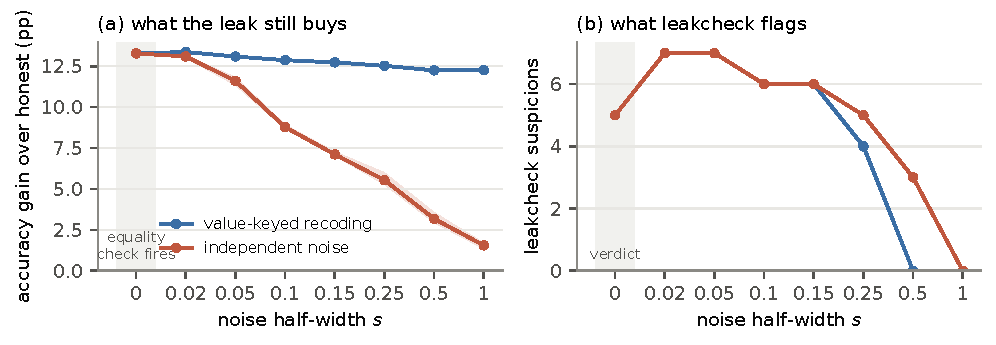
\includegraphics[width=0.92\textwidth]{fig11_detection_power.pdf}
\caption{\textbf{What gets through.} (a) Premium of the MRR@20 leak over honest features as the
noise half-width $s$ grows, for the value-keyed recoding and for independent additive noise of
$\pm s$ in absolute reward units (band: range over three noise draws). (b) \texttt{leakcheck}
suspicions on the same matrices; the only verdicts, like the only equality-check hits, are at
$s{=}0$.}
\label{fig:detect}
\end{figure}

\paragraph{Beyond our pipeline.} On RouterBench~\cite{hu2024routerbench} (2{,}553 strictly-won
queries), where label-free prompt features add only $+0.94$ points, exposing 1--8 models' rewards
buys $+16.2$ to $+63.7$, and 15\% multiplicative noise retains 92--98\% of it.

\paragraph{The leak persists at scale.} To test whether the effect depends on 500-passage
candidate sets, we rebuilt the pipeline on a single shared index, with no per-query candidate set
and no synthetic gold, at three corpus sizes from 20K to 100K passages (nested prefixes of one
seeded permutation). The leak's premium does not shrink as the corpus grows
(Figure~\ref{fig:scale}): leaked accuracy is flat at 63.4, 64.2 and 63.7\%, and the label-free
features stay below the majority baseline throughout. The premium rises by 1.4 points, but that
is within the cross-validation spread of a single seed, so we claim persistence, not growth.

\begin{figure}[t]
\centering
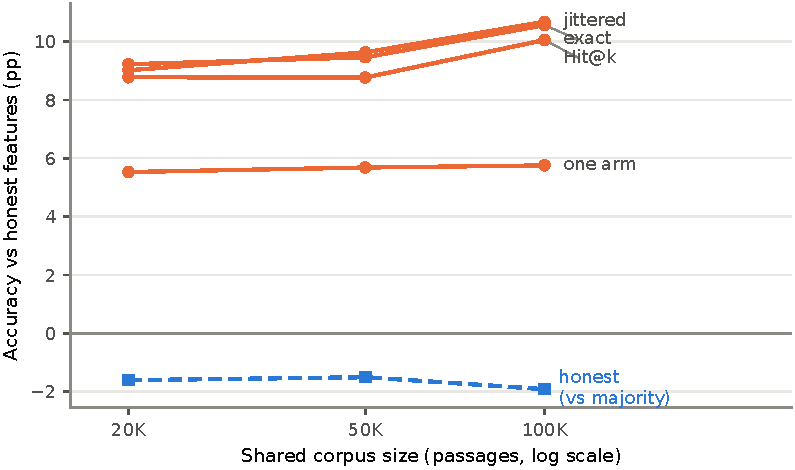
\includegraphics[width=0.66\textwidth]{fig10_leak_vs_scale.pdf}
\caption{Leak premium (accuracy minus that of label-free features) as one shared corpus grows from
20K to 100K passages, pooled over three datasets (2{,}918--3{,}634 informative queries). Exact leak
$+9.2 \to +10.6$, recoded $+9.0 \to +10.7$, honest features $-1.6 \to -1.9$. The leaked metric here
is MRR@5 (zero on 76--95\% of rows), so values are not comparable to Figure~\ref{fig:ladder}.}
\label{fig:scale}
\end{figure}

\paragraph{A gain is not proof of a leak.} In a synthetic task with genuine signal, boosting gains
$+14.0$/$+17.4$ points with no leak and 26--34 more with a noised leak (Supplementary~S1): the
two look alike.

% =====================================================================================
\section{RQ2: What remains without the leak?}
\label{sec:results}

\textbf{Takeaway: on these arms, nothing we tested beats the best fixed retriever, within a stated
detection limit.}

\paragraph{No method captures the headroom.} Table~\ref{tab:capture} scores every method on test
splits of 174/231/138 queries, against the best fixed retriever chosen in hindsight on the test
split (Dense throughout), the strongest fixed baseline. The largest capture is $+0.4\%$ (score-gap,
NQ; paired-bootstrap 95\% interval 0.0--1.5\%) and most are negative. Tuned gradient boosting
predicts the same arm as Always-Dense on 538 of 543 test queries. This matches the collapse to a
constant policy reported for LLM routers~\cite{garg2026unsolvability}. Further baselines (convex
fusion, a cost-aware cascade, PPO and GRPO, per-retriever reward regression) are in
Supplementary~S2; none holds up.

\begin{table}[t]
\centering
\small
\caption{Every method on the test split (reciprocal rank of the first answer-bearing passage).
Bold marks the best non-oracle value and implies no significance: no method beats the best fixed
retriever at $p<0.05$ (one-sided paired bootstrap; smallest $p{=}0.26$, for score-gap on NQ,
which changes one test query). RL: validation-selected
checkpoint, mean $\pm$ s.d.\ over 15 seeds.\protect\footnotemark{}}
\label{tab:capture}
\begin{tabular}{lccc}
\toprule
Routing strategy & NQ & TriviaQA & HotpotQA \\
\midrule
Always-BM25   & 0.1029 & 0.1501 & 0.0468 \\
Always-Dense  & 0.1655 & \textbf{0.2000} & \textbf{0.0753} \\
Always-Hybrid & 0.1464 & 0.1907 & 0.0572 \\
\midrule
Heuristic (score gap)      & \textbf{0.1657} & 0.1968 & 0.0753 \\
Logistic regression        & 0.1639 & 0.1990 & 0.0635 \\
Random forest              & 0.1640 & 0.1968 & 0.0753 \\
Ridge regression           & 0.1594 & 0.1981 & 0.0750 \\
Gradient boosting (tuned)  & 0.1642 & 0.2000 & 0.0753 \\
Policy-gradient RL         & $0.1618${\scriptsize$\pm$.0061} & $0.2000${\scriptsize$\pm$.0037}
                           & $0.0722${\scriptsize$\pm$.0036} \\
\midrule
Oracle & 0.2001 & 0.2694 & 0.1096 \\
\bottomrule
\end{tabular}
\end{table}
\footnotetext{Changed since review: the submitted version reported the RL policy's final-epoch
weights (0.1512/0.1881/0.0683), because the trainer never restored the selected checkpoint.}

\paragraph{Is there signal at all?} A router can be useless while its features still carry signal,
so we test against two nulls~\cite{ojala2010permutation} (Figure~\ref{fig:perm}). The honest
features beat both: shuffled labels give $59.1{\pm}0.2$ against the observed 59.9 ($p{=}0.003$), and
shuffling within each dataset moves the null by only 0.03 points ($p{=}0.016$, the floor at
$B{=}60$). \textbf{So the features carry some signal, but it stays 1.0 point below a constant
policy}, and no single dataset clears its own null. A better representation does not change
this: frozen query embeddings alone give 59.7\%, and score-distribution predictors in the style of
NQC~\cite{shtok2012nqc}, WIG~\cite{zhou2007wig} and SMV~\cite{tao2014smv} give $-1.34$ points.
Within these arms, the difficulty is in the label.

\begin{figure}[t]
\centering
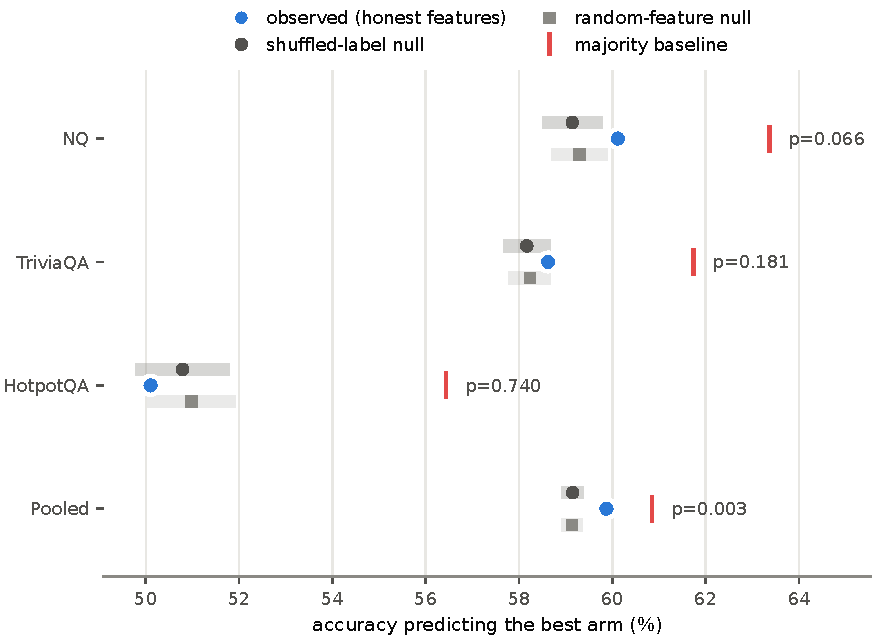
\includegraphics[width=0.78\textwidth]{fig9_permutation.pdf}
\caption{Honest features against two nulls: shuffled labels and random features; bands are
$\pm 1$ s.d.\ over $B{=}1000$ replicates, one-sided $p$ with floor 0.001. Pooled: 59.9 vs.\
$59.1{\pm}0.2$, $p{=}0.003$ (majority 60.9); random-feature null $p{=}0.002$. Per-dataset cells:
Supplementary~S2.}
\label{fig:perm}
\end{figure}

\paragraph{What the test could have detected.} On these test splits a router must capture
\textbf{68\%} (NQ), \textbf{43\%} (TriviaQA) or \textbf{72\%} (HotpotQA) of the headroom to be
distinguished from best fixed by a one-sided test at $\alpha{=}0.05$ with 80\% power. These
limits assume the oracle's per-query variance: a router that follows the oracle on a random
subset of queries is detectable from 47/20/54\%, while one that also switches wrongly needs more.
The test does have power against the effect of \S\ref{sec:doseresponse}: applied on the same
split to the tuned router trained on the exact leak (capture 48/70/64\%), it detects it on every
dataset (one-sided $p{=}0.016$, ${<}0.001$, $0.005$).
The oracle itself is partly an artifact: 16--22\% of headroom comes from
queries won by $\le 1\%$, and noise at 10\% of the reward's spread inflates it by 16--29\%, the
optimizer's curse of a maximum over noisy estimates~\cite{smith2006optimizerscurse}. We therefore
claim only that no method we tested reaches these limits; a router as good as those in
\S\ref{sec:related} could go undetected here.

% =====================================================================================
\section{RQ3: Can the leak be audited?}
\label{sec:tool}

\textbf{Takeaway: a feature matrix can be screened, but only an exact match is proof.}

We release \texttt{leakcheck}: given a feature matrix and a per-arm reward table, it reports which
columns carry reward information, without fitting a model. Its first design issued a verdict
whenever a feature's rank correlation with a reward passed a threshold calibrated on our leaks.
RouterBench falsified it: features built from prompt text alone, such as punctuation counts,
reached $|\rho|{=}0.881$ with zero exact agreement. RouterBench pools 86 benchmarks with different
prompt formats, so ``number of question marks'' identifies the benchmark, and the benchmark
predicts the winner~\cite{lee2026tasktype}. A confound through a shared cause looks exactly like a
monotone leak.

So \texttt{leakcheck} now issues \emph{verdicts} only on exact agreement, a fact about the arrays:
on more than 25\% of the rows where the reward is non-zero, or on every row when the reward is
binary. Rank-based findings are reported as \emph{suspicions}. The 25\% bar sits above every
honest column we measured (at most 6.1\%) and below our real leak (26--45\%), but a copy of a
more tightly truncated metric (MRR@5 against full-rank reciprocal rank) can fall under it. The
perturbed leaks of
Figure~\ref{fig:detect} are raised as suspicions, but a value-keyed recoding at $\pm$50\% or more
is missed, although gradient boosting still gains 12.3 points from it. An opt-in
test that predicts each arm's reward from one column on held-out rows, with a permutation
$p$-value, catches that case and labels a planted group confound in 10 of 10 trials. But it also
flags 91\% of genuinely predictive synthetic columns, including our honest overlap features. Any
check that catches perturbed leaks flags real signal too, because from the data alone a
predictive feature and a leak look the same. The tool gives triage; provenance settles whether a
column is legitimate, and an ablation measures what it was worth. Table~\ref{tab:bench} compares it with simpler checks on planted leaks.

\begin{table}[t]
\centering
\small
\caption{\textbf{Which check catches which leak.} Rate at which each detector flags a planted column
built from one arm's reward (synthetic, 20 features of which 3 carry genuine signal, $n{=}2000$, 10
seeds). The last three rows are not leaks, so any flag there is a false alarm. Equality: exact
agreement; Pearson: linear correlation; Importance: held-out permutation importance of a
gradient-boosting router. Full table with an AUC scan and more scenarios: Supplementary~S3.}
\label{tab:bench}
\begin{tabular}{lccccc}
\toprule
Planted column & Equality & Pearson & Importance & \texttt{leakcheck} verdict & Decode test \\
\midrule
exact copy                     & 1 & 1   & 1    & 1 & 1 \\
monotone (rank)                & 0 & 1   & 1    & 0 & 1 \\
independent noise $\pm$0.15    & 0 & 1   & 1    & 0 & 1 \\
order-scrambled recoding       & 0 & 0.2 & 1    & 0 & 1 \\
split over two columns         & 0 & 1   & 1    & 0 & 1 \\
\midrule
group confound (not a leak)    & 0 & 0   & 1    & 0 & 1$^\dagger$ \\
genuine-signal columns         & 0 & 0.67 & 0.85 & 0 & 0.91 \\
pure-noise columns             & 0 & 0   & 0.026 & 0 & 0 \\
\bottomrule
\end{tabular}

{\footnotesize $^\dagger$ labelled as a group confound, not a leak, in 10 of 10 seeds when the group id is supplied.}
\end{table}

The pattern is the paper's argument in miniature: the only check with no false alarms
(equality, or a \texttt{leakcheck} verdict) misses every perturbed leak, and every check that
catches them also fires on genuine signal.

\paragraph{The obligation falls on papers.} When we checked (August 2026), RouterBench,
RouterArena~\cite{routerarena2026}, LLMRouterBench~\cite{llmrouterbench2026} and
RAGRouter-Bench~\cite{bansal2026ragrouter} shipped no feature matrix, so no reader could run even
an equality check. QueryRoute~\cite{le2026queryroute} has since shipped both arrays for its
query-reformulation selector, so we audited them: on four datasets (43--1{,}406 queries, 484
features over 11 candidates, five released metrics), no feature equals any candidate's per-query
outcome on any row, and the strongest associations ($|\rho|{\le}0.51$ with ${\ge}300$ queries,
held-out $R^2{\le}0.26$) are shared across candidates and sit on label-free difficulty predictors,
the signature of genuine signal. Our own leak agreed exactly on 26--45\% of rows. A clean audit
cannot exclude a perturbed leak, but this is what a routing paper that ships its arrays makes
possible. We release ours\footnote{Code, artifacts and \texttt{leakcheck}~0.2.1: \url{https://github.com/Soumya080/metric-feature-leakage} (start at \texttt{REVIEWERS.md}).}
and propose a checklist for routing papers, a routing-specific form of Kaufman et al.'s
legitimacy tags~\cite{kaufman2012leakage} and Kapoor and Narayanan's model info
sheets~\cite{kapoor2023leakage}: (1)~release the feature matrix $X$, the per-arm reward table
$R$ and the split identifiers; (2)~tag every column with when it becomes available: before any
arm runs (query only), after an arm runs but before the outcome is known (label-free arm
statistics, legal only if the policy pays for that arm), or after the outcome (computed from the
gold answer: never a feature); (3)~screen $X$ against $R$ for exact agreement and for
decodability, and for non-binary rewards also for rank agreement, knowing that the last two also
flag genuine signal; (4)~ablate every flagged column and report the result with and without it;
(5)~report the smallest capture the test split could detect next to any claimed gain. Items
(2)--(5) are also a reader's questions, any one of which would have caught our bug, and none needs
the authors' code, only their feature matrix.

% =====================================================================================
\section{Discussion: what this means beyond our router}
\label{sec:discussion}

\paragraph{Why the failure is easy to make and hard to see.} Three conditions produced it, and
none is specific to our code. Evaluation metrics were stored next to label-free statistics in the
same record, because the same retrieval run produces both. The leaked feature had a plausible name
and a plausible range. And the honest alternative performed \emph{worse} than a constant baseline,
so every signal a researcher normally trusts, a better score and a simpler model that still
works, pointed toward the leak. Any pipeline that logs evaluation results per query and later
mines that log for features meets the first two conditions.

\paragraph{Where else it applies.} The mechanism needs only a per-arm reward table and features
built from the same logs: LLM routing, where per-model correctness is logged per prompt (our
RouterBench injection buys up to $+63.7$ points); algorithm selection, whose closed-gap metric
capture is; and model cascades and adaptive retrieval generally. We have measured it in one
setting and injected it into one other; how often it occurs in published work is open, and
cannot be measured until feature matrices are released.

% =====================================================================================
\section{Limitations}
\label{sec:limitations}

\begin{itemize}\setlength{\itemsep}{1pt}\setlength{\parskip}{0pt}
  \item \textbf{One pipeline.} The leak occurred naturally once, in our pipeline; the other rungs
    are constructed and vary coverage and fidelity together rather than one measured quantity.
  \item \textbf{Weak, Dense-dominated arms.} Hybrid is redundant, BM25 is handicapped by the
    candidate sets, and Dense was fine-tuned on NQ and TriviaQA questions; on a shared index the
    ordering changes (\S\ref{sec:setup}). A larger, more diverse pool would test routing properly.
  \item \textbf{Proxy reward and query-side features.} Answer-string reciprocal rank is not answer
    quality: 27--46\% of our queries have answer-bearing distractors (Supplementary~S2; cf.\ the
    unjudged-relevant problem of shallow pools~\cite{arabzadeh2022shallow}), and gold is
    answer-string presence in a 100K-passage sample, which keeps 46--81\% of queries and favours
    common answers. No feature reads the retrieved text, where post-retrieval
    routers~\cite{qin2024ltrr,zhao2026r3ag,six2026ragcompass} find signal, and we judge routing
    only on effectiveness, not on the cost at matched effectiveness that motivated it in
    IR~\cite{arabzadeh2021bertselect}.
  \item \textbf{Power.} No per-dataset null clears $\alpha{=}0.05$; Table~\ref{tab:capture} uses one
    small split~\cite{fuhr2017mistakes}; the detection limits above bound every negative claim.
\end{itemize}

% =====================================================================================
\section{Conclusion}

A learned router appeared to beat fixed retrieval because four of its sixty-one features were
read from the evaluation metric. That leak buys most of the oracle gap, survives a change of
metric and, partly or fully depending on its form, noise, so an equality check does not catch it.
Without it, nothing we tested beats committing to one retriever on these arms. We do not conclude
that routing cannot work. We conclude that a routing result should ship with its feature matrix,
and that the matrix should be checked before the result is believed.

\bibliographystyle{plain}
\bibliography{references}

\end{document}
